\chapter{Konzeptuelle Lösung / Umsetzung - Plesynd} 
\label{chapter:Kapitel5}
\lhead{Kapitel 5 \emph{Konzeptuelle Lösung / Umsetzung - Plesynd}}  
Das Ziel dieser Arbeit ist der Entwurf und die prototypische Implementierung einer leichtgewichtigen Personal Learning Environment mit Offline"=Funktionalitäten auf Basis aktueller Technologien, welche die Anforderungen aus Kapitel \ref{chapter:Kapitel3} erfüllt. 

Der Name des entwickelten Systems lautet \emph{Plesynd} (Personal Learning Environment Synchronize Data) und wird wie das englische "`pleasant"' (angenehm) ausgesprochen. Plesynd ist ein webbasiertes Dashboard, welches die Möglichkeit bietet mit unterschiedlichen Widgets in Kommunikation zu treten. Wichtig ist hierbei eine Abgrenzung zu zentralisierten Lern"=Management"=Systemen wie Moodle oder Sakai. Die sind sehr kurszentriert und entsprechen nicht dem nutzerzentrierten Ansatz von Personal Learning Environments. Aus diesem Grund orientiert sich Plesynd viel stärker an bestehenden Widget"=Aggregatoren wie iGoogle oder Netvibes (siehe Abschnitt \ref{section:aehnliche_systeme}). In einem nutzerzentrierten Ansatz, muss dem Anwender die Möglichkeit gegeben werden in unterschiedlichen Kontexten mit dem System zu arbeiten. Hierzu erlaubt es Plesynd dem Anwender seine Widgets in einer frei wählbaren Anzahl unterschiedlicher Bereiche, sogenannter Workspaces, aufzuteilen. Der entscheidende Unterschied von Plesynd zu den erwähnten Systemen ist die Offline"=Fähigkeit der PLE. Es wurde ein Ansatz entwickelt, der es ermöglicht das System auch ohne Internetverbindung zu starten und Widgets so zu implementieren, dass ihre Informationen offline verfügbar gemacht werden und offline mit Plesynd und den Widgets weitergearbeitet werden kann. Sobald der Browser wieder eine Online"=Verbindung hergestellt hat, werden die veränderten Daten mit dem Backend synchronisiert. Zusätzlich zu dem Grundsystem von Plesynd wurde in dieser Arbeit ein Todo"=Listen Widget entwickelt, welches die erwähnten Funktionalitäten nutzt und zeigt wie dem System zusätzliche Widgets hinzugefügt und komplett in Plesynd integriert werden können. Das komplette entwickelte System, inklusive der benötigten Komponenten, wurde der Arbeit als CD beigefügt. Eine Installationsanleitung befindet sich im Anhang.

Das vorliegende Kapitel liefert einen Überblick über die grundsätzliche Architektur von Plesynd und seiner Komponenten und eine Beschreibung des implementierten User"=Interfaces.

% \begin{landscape}
\begin{figure}
  \centering
  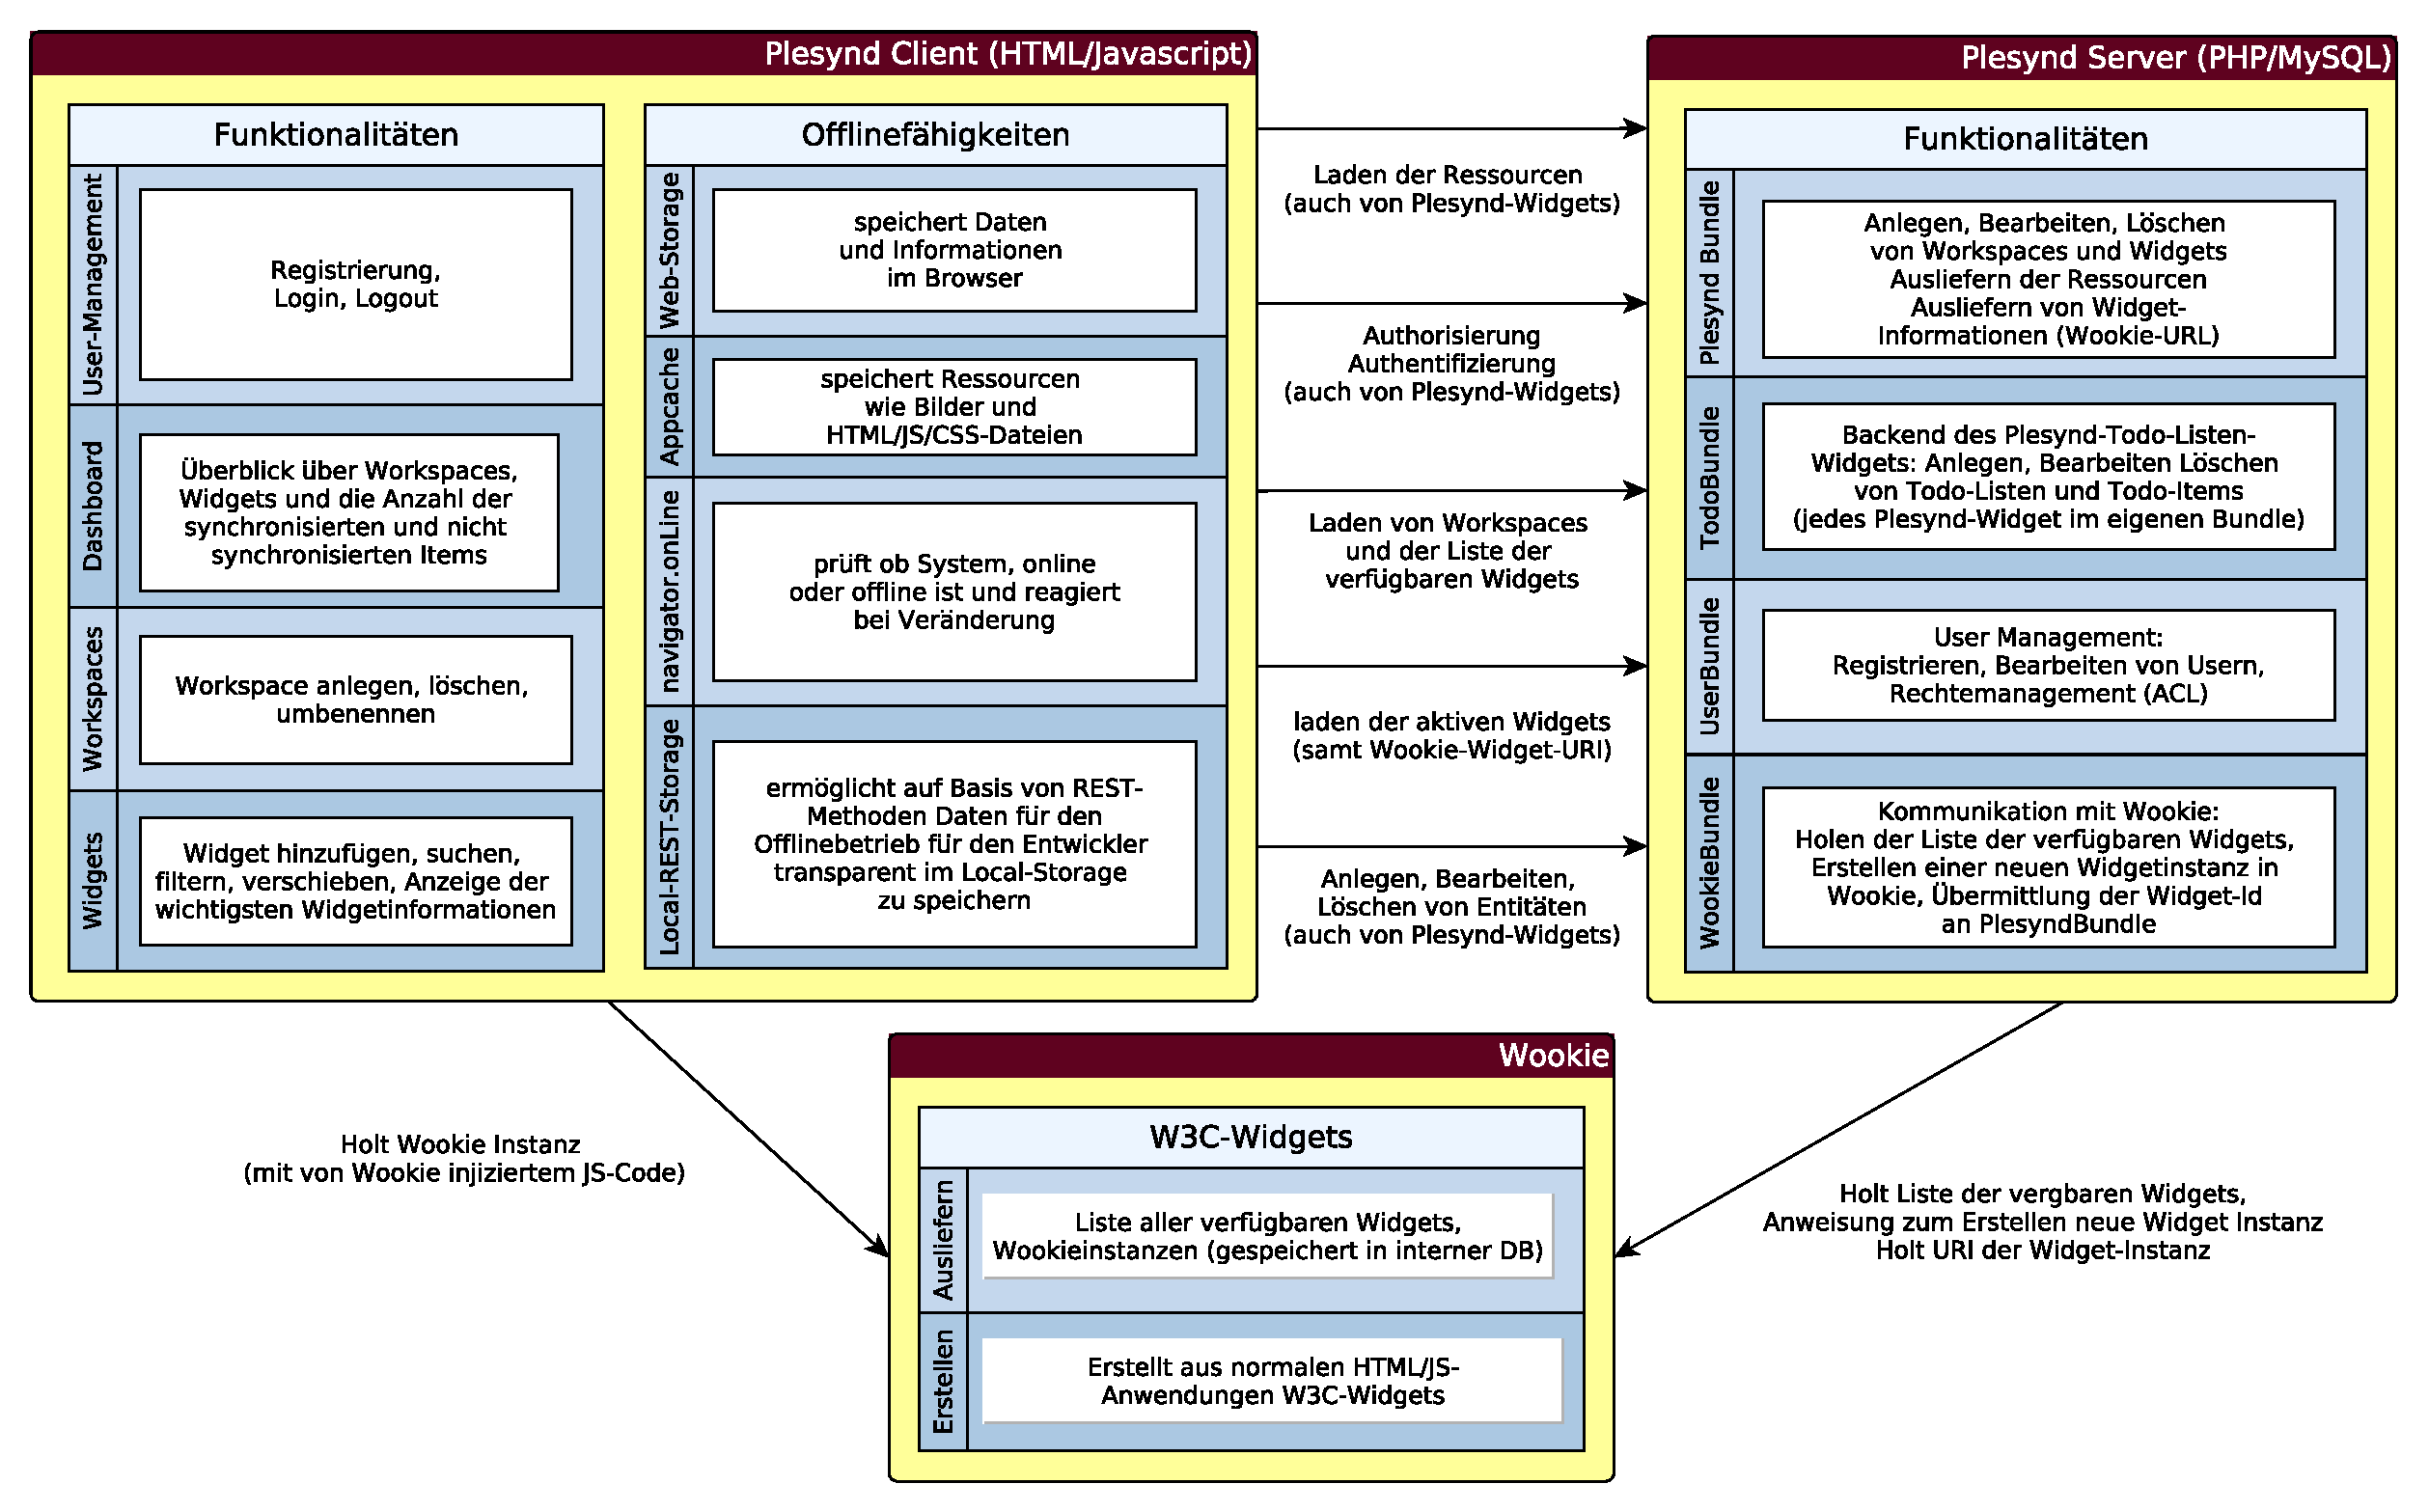
\includegraphics[width=\textwidth,keepaspectratio]{./Figures/konzeptionelle_loesung_table.pdf}
    \rule{35em}{0.5pt}
  \caption[Überblick über die Komponenten von Plesynd]{Überblick über die Komponenten von Plesynd}
  \label{fig:ueberblick_plesynd_komponenten}
\end{figure}
% \end{landscape}

\section{Überblick über die Architektur von Plesynd}\label{section:plesynd_architektur}
Zunächst gibt Abbildung \ref{fig:ueberblick_plesynd_komponenten} einen Überblick über die wichtigsten Komponenten des entwickelten Systems und über deren Zusammenspiel. Plesynd selbst besteht aus zwei Komponenten, Plesynd"=Client und Plesynd"=Server. Diese liefern zusammen die Funktionalitäten, welche die gestellten Anforderungen erfüllen sollen. Zusätzlich wird Wookie als externe Komponente zum Ausliefern und Erstellen der Widgets verwendet.

\subsection{Plesynd-Client}
\begin{figure}
  \centering
  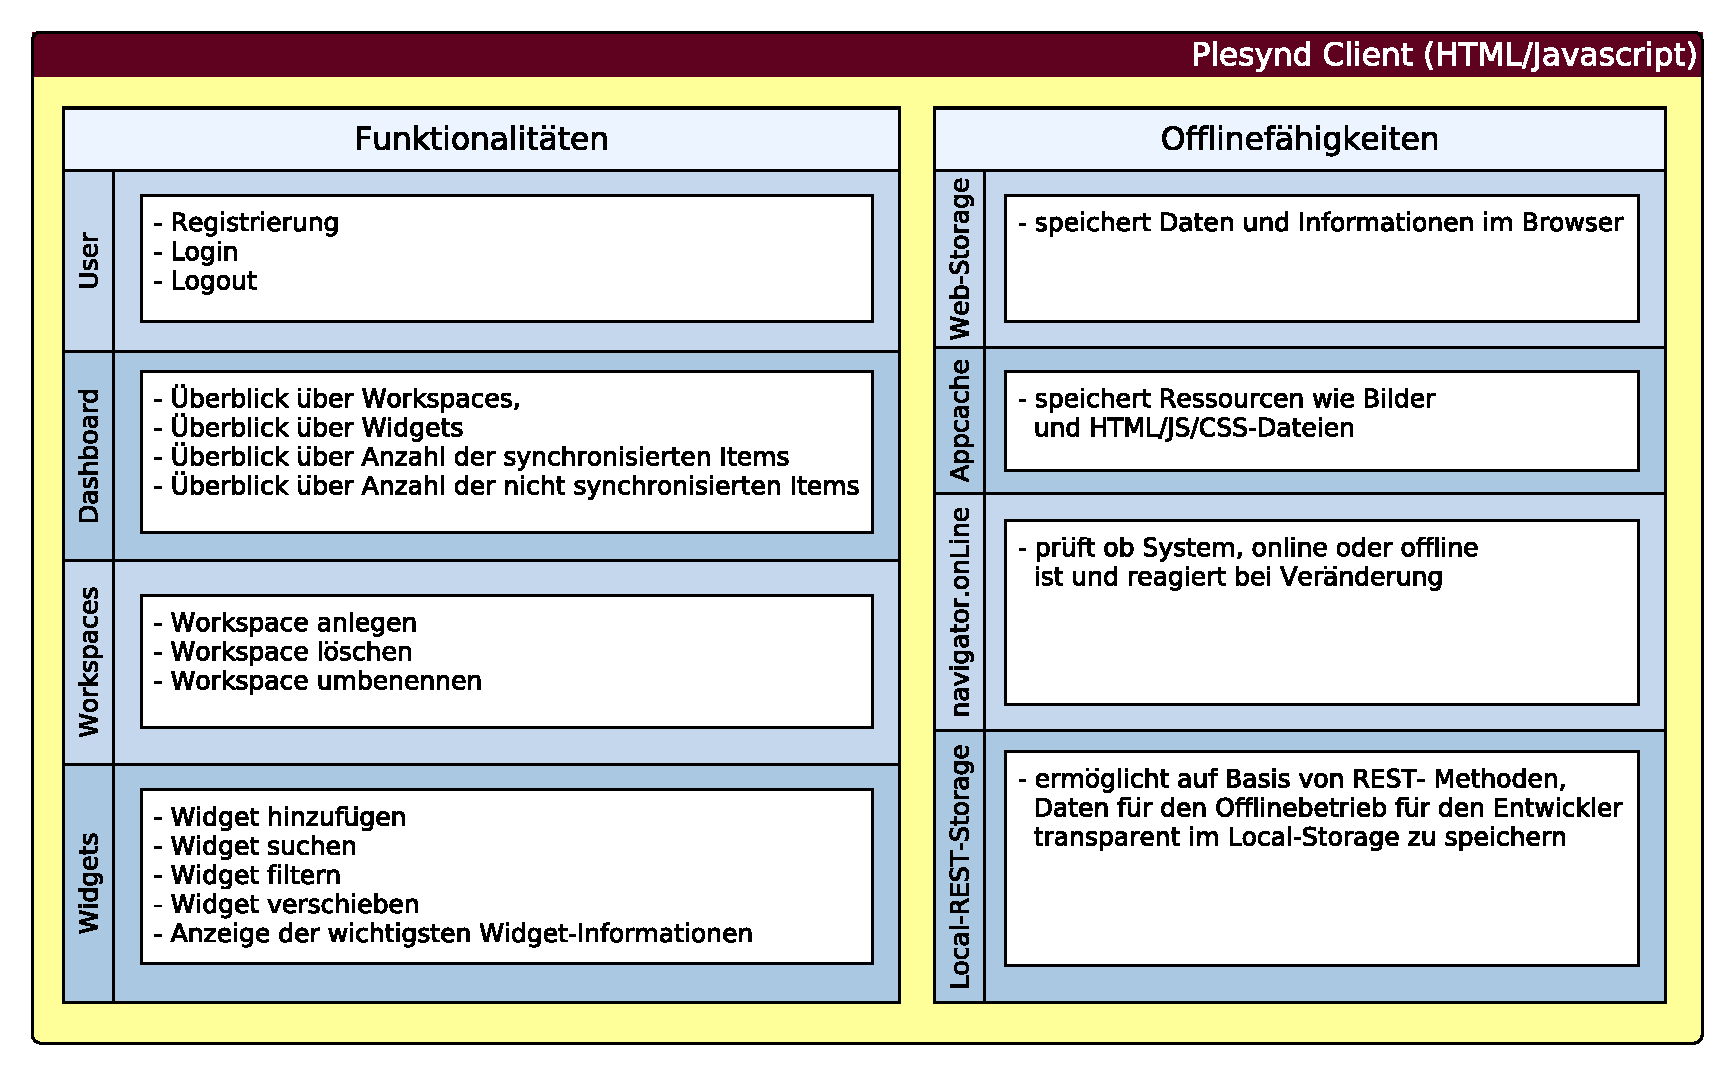
\includegraphics[height=10cm,keepaspectratio]{./Figures/konzeptionelle_loesung_plesynd_client.pdf}
    \rule{35em}{0.5pt}
  \caption[Überblick Plesynd-Client]{Überblick Plesynd-Client}
  \label{fig:ueberblick_plesynd_client}
\end{figure}
Plesynd"=Client (siehe Abbildung \ref{fig:ueberblick_plesynd_client}) bezeichnet den Teil der Anwendung, der direkt beim Client, also im Browser des Anwenders läuft. Diese Komponente umfasst den größten Teil des entwickelten Systems und ist auch für die Offline"=Funktionalitäten von Plesynd verantwortlich. Plesynd"=Client stellt über ein User"=Interface den Teil der PLE dar, mit dem der Anwender direkt in Berührung kommt. Es liefert Funktionalitäten zum Anlegen und Bearbeiten von Workspaces, versetzt den Anwender in die Lage nach Widgets zu filtern, diese den Workspaces hinzuzufügen und neu anzuordnen und stellt ihm ein Dashboard zur Verfügung auf dem die wichtigsten Informationen zu seinen Workspaces und Widgets zusammengefasst werden. Es informiert den Nutzer auch darüber, ob das System eine Verbindung zu dem Internet hat oder nicht. Zusätzlich gibt es dem Anwender die Möglichkeit sich zu registrieren und sich in das System einzuloggen. 

Die Fähigkeit von Plesynd und des Todo"=Listen"=Widgets Anwendungsdaten offline vorzuhalten wurde auf Basis der Web"=Storage Technologie entwickelt (siehe Abschnitt \ref{section:offline_storage}). Plesynd erkennt über ein globales Javascript"=Event (siehe Abschnitt \ref{section:online_offline_erkennung}), wenn sich der Browser in einem Zustand befindet, in dem er keine Konnektivität mit dem Internet besitzt. Das System informiert den Anwender darüber, kann aber auch entscheiden, welche Funktionalitäten es dem Nutzer nur noch eingeschränkt zur Verfügung stellt. Nimmt der Anwender Änderungen an den Daten vor, werden diese in den Local"=Storage geschrieben. Sobald sich das System wieder mit dem Internet verbindet, erkennt Plesynd diese Zustandsänderung und synchronisiert die Daten mit den zugrunde liegenden Services. Sollte einmal eine andere Speichertechnik als der Web"=Storage benötigt werden, ist das System so implementiert, dass die Art der lokalen Speicherung losgelöst von der restlichen Anwendung umgestaltet werden kann. Entwickelt wurde diese Funktionalität mit besonderem Augenmerk auf die Implementierung zusätzlicher Widgets. Dies bedeutet, dass auf Basis der vorliegenden Implementierung mit relativ wenig Aufwand weitere Widgets für unterschiedliche Services erstellt werden können. Die Art des Services ist nicht von Belang. Er sollte nur in der Lage sein einfache REST"=Anfragen (siehe Abschnitt \ref{section:rest}) zu verstehen, zu verarbeiten und standardkonform auf sie zu antworten. Die Möglichkeit, Ressourcen wie Javascript, CSS und HTML Dateien im Browser zu speichern, wurde mit der HTML5 Appcache"=API umgesetzt (siehe Abschnitt \ref{section:appcache}). Probleme, mit der bei modernen Browser üblichen Same"=Origin"=Policy (siehe Abschnitt \ref{section:same_origin_policy}) für Requests, wurden mit dem Cross"=Origin Resource Sharing (CORS) Mechanismus und der Postmessage"=API gelöst. 

\subsection{Plesynd-Server}
\begin{figure}
  \centering
  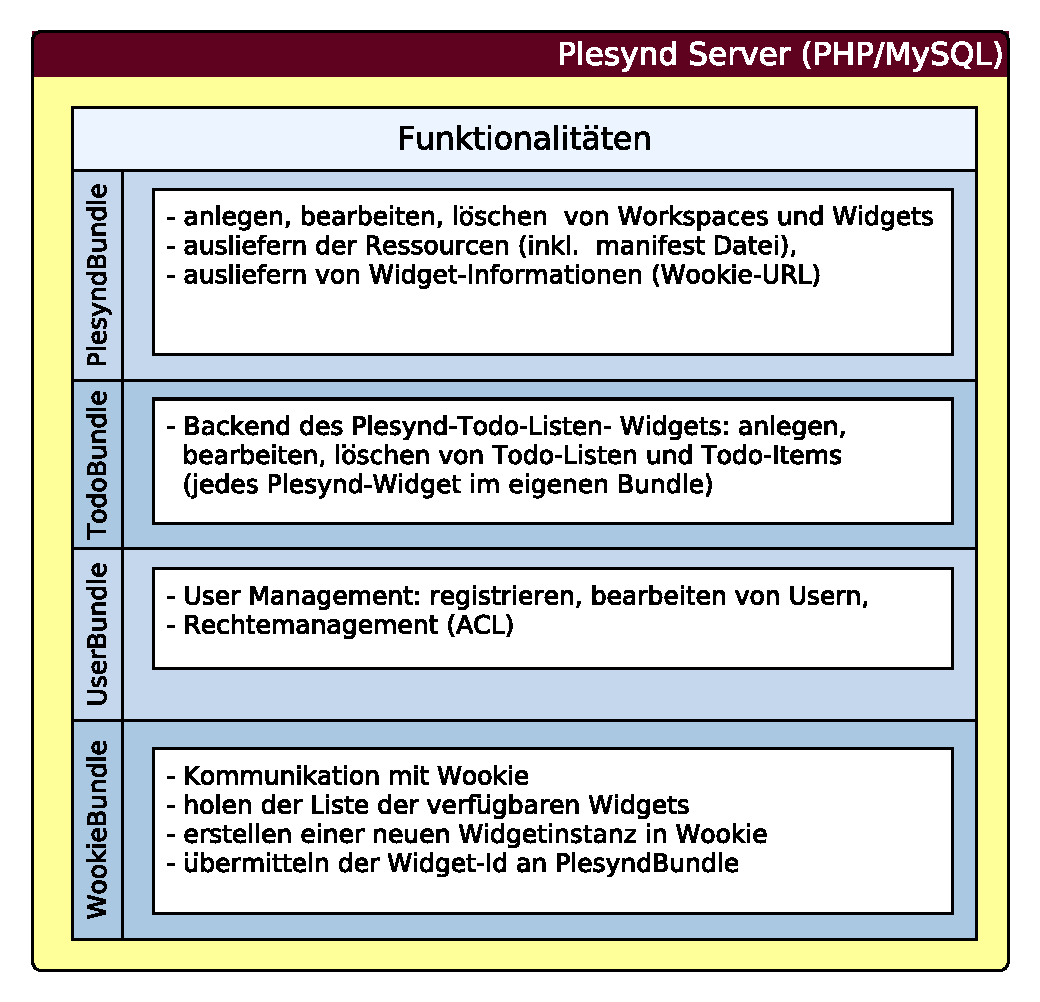
\includegraphics[height=10cm,keepaspectratio]{./Figures/konzeptionelle_loesung_plesynd_server.pdf}
    \rule{35em}{0.5pt}
  \caption[Überblick Plesynd-Server]{Überblick Plesynd-Server}
  \label{fig:ueberblick_plesynd_server}
\end{figure}
Plesynd"=Client ist, wie eben beschrieben, in der Lage sowohl Ressourcen als auch Daten lokal beim Client zu speichern und so auch offline verfügbar zu machen. Es benötigt zum normalen Betrieb aber ein Backend, welches diese Ressourcen initial ausliefert und sich um die persistente Speicherung der Daten und das Rechtemanagement kümmert. Für diesen Zweck wurde die Plesynd"=Server Komponente (siehe Abbildung \ref{fig:ueberblick_plesynd_server}) entworfen. Diese Komponente besteht aus mehreren Bundles (siehe Abschnitt \ref{section:symfony2}), wobei jedes Bundle für einen bestimmten Aufgabenbereich innerhalb  von Plesynd"=Server zuständig ist. Aufgaben von Plesynd"=Server sind das Ausliefern der Ressourcen, die Speicherung von Workspace und den zugehörigen Widgets samt ihrer Position auf dem Workspaces, das User"=Management (Registrierung, Login etc) und das Rechtemanagement, also die Prüfung welcher Nutzer Zugriff auf welchen Workspace, Widget oder welche Todo"=Liste hat. 

Plesynd"=Server nimmt für die Arbeit mit den Anwendungsdaten (Workspace, Widgets, Todo"=Listen etc.) REST konforme Anfragen (siehe Abschnitt \ref{section:rest}) entgegen und antwortet standardkonform.

Für die Abfrage welche Widgets grundsätzlich im System vorhanden sind verwendet Plesynd"=Server eine Schnittstelle zur Wookie"=Komponente. Diese Schnittstelle wird auch verwendet wenn der Anwender ein neues Widget zu einem Workspace hinzufügen möchten, also eine neue Widget"=Instanz erstellt werden muss.

\subsection{Wookie}\label{section:loesung_wookie}
\begin{figure}[ht]
  \centering
  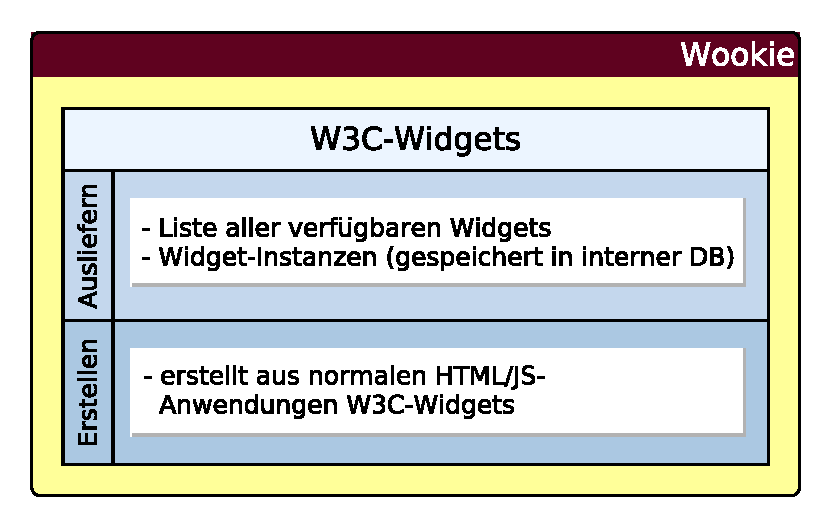
\includegraphics[height=5cm,keepaspectratio]{./Figures/konzeptionelle_loesung_wookie.pdf}
    \rule{35em}{0.5pt}
  \caption[Überblick Wookie]{Überblick Wookie}
  \label{fig:ueberblick_wookie}
\end{figure}
Als externe Komponente wird der W3C"=Widget"=Container Wookie (siehe Abbildung \ref{fig:ueberblick_wookie} und Abschnitt \ref{section:widget_frameworks}) eingebunden. Dieser speichert die verfügbaren Widgets in einer internen Datenbank und kann Plesynd so eine Liste der auslieferbaren Widgets zur Verfügung stellen. Wookie hinterlegt außerdem jede einzelne erstellte Widget"=Instanz samt ihrem Zustand und kann so das eigentliche Widget bei Bedarf an Plesynd"=Client ausliefern. Diese Funktionalität ist die einzige, bei der Plesynd"=Client direkt Kontakt zu Wookie aufnimmt, ansonsten wird die gesamte Kommunikation über Plesynd"=Server abgewickelt. Zusätzlich zu diesen Anwendungsfällen bietet Wookie Werkzeuge an, um aus normalen HTML/Javascript"=Applikationen ein W3C"=Widget zu erstellen. Diese Funktionalität steht jedoch nicht über die Kommunikation mit Plesynd zur Verfügung, sondern muss über die Kommandozeile in Anspruch genommen werden.

\section{Umsetzung}\label{section:umsetzung}

Die für die Umsetzung implementierten Funktionalitäten orientieren sich an den in Abschnitt \ref{section:anwendungsfaelle} definierten funktionalen Anforderungen. Für die Umsetzung der Screen"=Dimension (siehe Abschnitt \ref{section:dimensions_palmer}), also des User"=Interfaces kommen in Plesynd drei wichtige Konzepte zum Einsatz: Dashboard, Widgets und Workspaces. Über Widgets werden die unterschiedlichen Werkzeuge und Services, die ein Nutzer innerhalb des Systems nutzen möchte eingebunden (siehe Abschnitt \ref{section:widgets}). Die Umsetzung der einzelnen Widgets liegt in der Hand des jeweiligen Designers. Da Plesynd Wookie als Widget Container benutzt, ist es möglich alle W3C"=Widgets in das System einzubinden. Für diese Arbeit wurde ein Todo"=Listen"=Service entwickelt für den als prototypische Entwicklung ein Widget mit Online"=/Offline"=Fähigkeiten implementiert wurde. Besitzt ein Widget Online"=/Offline"=Fähigkeiten so erhält es eine von Plesynd zur Verfügung gestellte Statusleiste, in der der aktuelle Online"=/Offline"=Status sowie die Anzahl der verfügbaren Einträge und der noch nicht synchronisierten Einträge angezeigt wird (siehe Abbildungen \ref{fig:plesynd_workspace_online} und \ref{fig:plesynd_workspace_offline}). Der Nutzer hat die Möglichkeit Widgets nach Themen oder Einsatzgebieten zu gruppieren. Dies geschieht über sogenannte Workspaces. Workspaces sind vom Nutzer frei und in unbegrenzter Zahl hinzufügbare Bereiche im System. Sie sind über eine Reiter"=Navigation zu erreichen und können jederzeit umbenannt oder auch wieder gelöscht werden (siehe Abbildung \ref{fig:plesynd_workspace_edit}). Im folgenden werden die Umsetzungen der einzelnen Anforderungen genauer betrachtet.

Für die Umsetzung von Anforderung \reqref{requirementRegistrieren} (\emph{\requirementRegistrieren}) wurde eine Registrierungmechanismus implementiert. Ist der Anwender noch nicht registriert, hat er die Möglichkeit ein Anmeldeformular (siehe Abbildung \ref{fig:plesynd_register}) auszufüllen und dieses an den Server zu senden. Die gesendeten Daten werden validiert und führen im Fehlerfall zu einer erneuten Darstellung des Formulars samt Fehlermeldung und im Erfolgsfall zu einer Mitteilung an den Anwender, dass er sich als neuer Nutzer von Plesynd registriert hat. Abbildung \ref{fig:plesynd_register} zeigt ebenfalls die Umsetzung der Anforderung \reqref{requirementUniqueLoginEmail} (\emph{\requirementUniqueLoginEmail}). Zur Umsetzung von Anforderung \reqref{requirementLogin} (\emph{\requirementLogin}) hinterlegt Plesynd-Server die registrierten Anwender in einer Datenbank. Plesynd-Client bietet dem Nutzer die Möglichkeit sich über ein Formular an dem System anzumelden und anschließend mit ihm zu arbeiten (siehe Abbildung TODO).
Für Anforderung \reqref{requirementZugriffAufEigeneWidgets} (\emph{\requirementZugriffAufEigeneWidgets}) benutzt Plesynd, wie Abbildung \ref{fig:ueberblick_plesynd_server} zeigt, auf Serverseite Access-Control-Lists und hinterlegt damit für jeden Workspace und jedes Widget welcher Anwender diese erstellt und damit auch Zugriff auf sie hat. Andere Nutzer erhalten, auch wenn sie den Link zu einem Workspace kennen keinen Zugriff darauf. Ähnliches gilt ebenso für die mit Hilfe des Todo-Listen-Widgets erstellten Todo-Listen und Todo-Einträge. Klickt der Anwender auf den Link Logout (siehe Abbildung \ref{fig:plesynd_dashboard}), beendet das System seine Session und leitet ihn wieder auf die Login-Seite um. Dies stellt eine Umsetzung der in \reqref{requirementLogout} (\emph{\requirementLogout}) geforderten Funktionalität dar. Klickt der Anwender auf den Logout-Link, so wird seine Session auf dem Server beendet. Dies bedeutet, dass jeder weitere Request zu einem Fehler (403-Error) führt, welcher das System dazu veranlasst dem Anwender erneut die Login-Seite zu präsentieren. Es ist somit kein weiterer Zugriff auf die Daten möglich, was eine Realisierung von Anforderung \reqref{requirementKeinZugriffNachLogout} (\emph{\requirementKeinZugriffNachLogout}) darstellt. Zur Umsetzung von Anforderung \reqref{requirementWorkspaceAdd} (\emph{\requirementWorkspaceAdd}) wurde ein Hinzufügen Button in der Reiternavigation des Systems (siehe Abbildung \ref{fig:plesynd_dashboard}) implementiert, welcher direkt einen neuen Workspace zu dem System hinzugefügt.  \reqref{requirementWorkspaceEdit} (\emph{\requirementWorkspaceEdit}) fordert das Bearbeiten von Workspaces. Hierzu befindet sich in der genannten Reiternavigation neben einem aktiven Workspace ein Icon (siehe Abbildung \ref{fig:plesynd_workspace_edit}). Aktiviert der Anwender dieses, öffnet sich ein Bereich zum Bearbeiten des Workspaces. In diesem kann der Name direkt geändert werden. In dem Bereich zum Ändern des Workspace befindet sich auch ein Button zum Löschen desselben (siehe Abbildung \ref{fig:plesynd_workspace_edit}). Klickt der Anwender auf diesen, so wird ihm ein Rückfragefenster präsentiert. Bestätigt er hier das Löschen, wird der Workspace samt seiner Widgets aus dem System entfernt. Dies stellt eine Realisierung von Anforderung \reqref{requirementWorkspaceDelete} (\emph{\requirementWorkspaceDelete}) dar. \reqref{requirementWidgetAdd} (\emph{\requirementWidgetAdd}), \reqref{requirementWidgetFilterName} \emph{\requirementWidgetFilterName} und \reqref{requirementWidgetFilterOnline} \emph{\requirementWidgetFilterOnline} werden folgendermaßen realisiert: Im Bereich zum Bearbeiten eines Workspaces wird dem Anwender eine Maske zum Hinzufügen von Widgets angezeigt (siehe Abbildung \ref{fig:plesynd_workspace_edit}). Hier ist es ihm möglich ein Widget aus der Liste der zur Verfügung stehende Widgets auszuwählen. Wird ein Widget ausgewählt, werden dem Anwender die wichtigsten Informationen zu diesem Widget präsentiert. Bei Klick auf einen Button zum Hinzufügen wird das ausgewählte Widget an der nächste freien Position dem Workspace angehängt. Plesynd-Client bietet dem Anwender in der Maske zum Hinzufügen von Widgets einen eigenen Bereich an, in dem nach dem Namen des Widgets gesucht werden kann (siehe Abbildung \ref{fig:plesynd_workspace_edit}). Diese Suche findet nur auf dem Client statt, sendet also keine weiteren Anfragen an Plesynd-Server. Der Suchbereich, enthält neben dem Suchfeld noch einen Filter-Button, der es erlaubt nur offline-fähige Widgets anzuzeigen (siehe Abbildung \ref{fig:plesynd_workspace_edit}). Diese Filterung findet wie die Suche nur auf dem Client statt. Zum Löschen eines Widgets (Anforderung \reqref{requirementWidgetDelete} \emph{\requirementWidgetDelete}) kann der Anwender auf einen Button in der Widget-Statusleiste (siehe Abbildung \ref{fig:plesynd_workspace_edit}) oder auf dem Dashboard (siehe Abbildung \ref{fig:plesynd_dashboard}) klicken. Ihm wird anschließend wird ein Rückfragefenster präsentiert. Bestätigt er hier das Löschen, wird das Widget aus dem Workspace und damit auch aus dem System entfernt. Befindet sich der Anwender auf einem Workspace und hat dieser Workspace mehr als ein Widget, so ist der Anwender in der Lage mit einem Klick auf die Widget-Statusleiste die Widgets per Drag and Drop auf dem Workspace neu anzuordnen. Die neuen Positionen werden direkt an den Server weitergegeben und somit persistiert (siehe Abbildung TODO). Dies stellt eine Umsetzung der in \reqref{requirementWidgetSortDragNDrop} (\emph{\requirementWidgetSortDragNDrop}) Drag and Drop Funktionalität dar. Zur Umsetzung der Anforderungen \reqref{requirementWidgetInformSystem} (\emph{\requirementWidgetInformSystem}) und \reqref{requirementWidgetInformUser} (\emph{\requirementWidgetInformUser})  wurde folgendermaßen vorgegangen: Wenn der Anwender ein Plesynd-kompatibles Widget zu einem Workspace hinzufügt, meldet sich dieses bei Plesynd an und kann es über die Anzahl der verfügbaren und synchronisierten und nicht synchronisierten Einträge informieren (siehe Abbildung TODO). Diese Funktionalität wurde über die Postmessage-API implementiert (siehe Abschnitt \ref{section:kommunikation_in_mashup_anwendungen}). Als Startseite von Plesynd wurde ein Dashboard umgesetzt, welches die Workspaces samt ihrer Widgets auflistet (siehe Abbildung \ref{fig:plesynd_dashboard}). Für jedes Widget erhält der Anwender die Information, ob es Plesynd-kompatibel ist. Falls dem so ist, werden dem Anwender angezeigt wie viele Einträge vorhanden und wie viele synchronisiert und nicht synchronisiert sind. Zusätzlich kann der Anwender über das Dashboard Widgets entfernen und sich über Links direkt zu den gewünschten Workspaces bewegen. Dieses Dashboard dient zur Realisierung von Anforderung \reqref{requirementDashboard} (\emph{\requirementDashboard}).

Die Anforderungen \reqref{requirementCheckOnlineStatus} (\emph{\requirementCheckOnlineStatus}), \reqref{requirementOnlineStatusInformUser} (\emph{\requirementOnlineStatusInformUser}), \reqref{requirementOfflineStart} \emph{\requirementOfflineStart}, \reqref{requirementOfflineWork} (\emph{\requirementOfflineWork}) und \reqref{requirementOnlineSync} (\emph{\requirementOnlineSync}) beschreiben die erforderlichen offline Funktionalitäten des Systems. Plesynd nutzt die in Abschnitt \ref{section:online_offline_erkennung} beschriebene Online-/Offline-Erkennung für die Umsetzung von Anforderung ). Der aktuelle Status wird dem Nutzer direkt im System (siehe Abbildung \ref{fig:plesynd_dashboard}) und bei Plesynd-kompatiblen Widgets (siehe Abbildung \ref{fig:plesynd_workspace_offline}) angezeigt. Plesynd-Client speichert mit Hilfe der HTML-Appcache-API (siehe Abschnitt \ref{section:appcache}) die benötigten Ressourcen beim erstmaligen Systemstart im Browser. Ab diesem Zeitpunkt ist es möglich das System auch ohne Online-Verbindung zu laden. Abbildung TODO zeigt, wie die Workspace und Widgets im Local-Storage hinterlegt werden. Mit Hilfe der in Abschnitt \ref{section:offline_storage} beschriebenen Techniken und der entwickelten Systematik zum Speichern und Synchronisieren von Daten (siehe Abschnitt \ref{section:offline_faehigkeiten}), ist es möglich mit Plesynd-Client und den kompatiblen Widgets offline zu arbeiten. Das System synchronisiert die hinzugefügten, geänderten und gelöschten Einträge mit den jeweiligen Backends, wenn wieder eine Verbindung zum Internet hergestellt wurde.


\begin{figure}[hb]
  \centering
  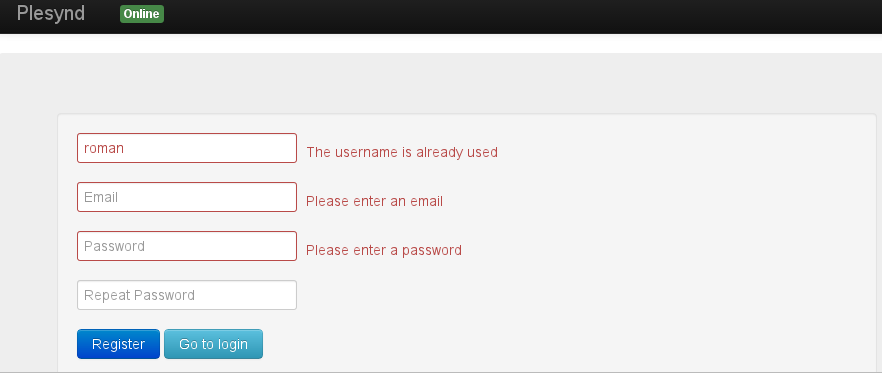
\includegraphics[]{./Figures/plesynd_register.png}
    \rule{35em}{0.5pt}
  \caption[Plesynd User"=Interface: Registrieren]{Der Anwender kann sich für die Nutzung von Plesynd registrieren}
  \label{fig:plesynd_register}
\end{figure}

\begin{figure}
  \centering
  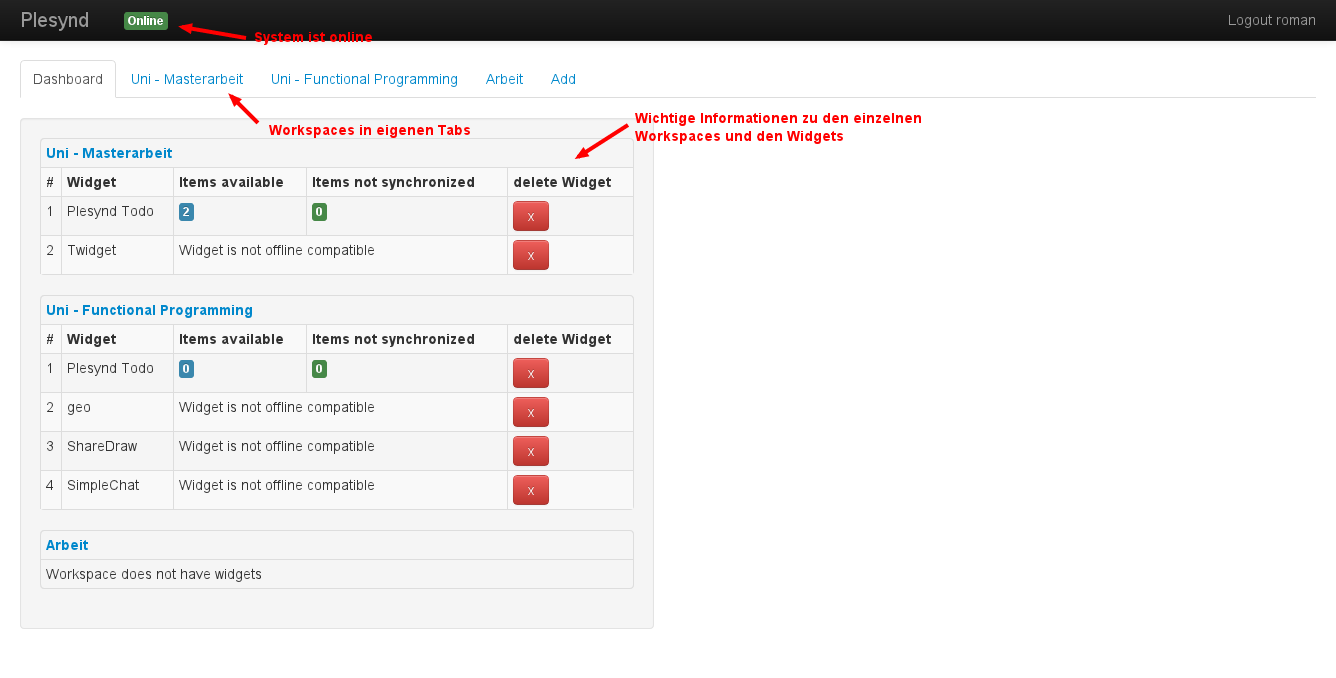
\includegraphics[]{./Figures/plesynd_dashboard.png}
    \rule{35em}{0.5pt}
  \caption[Plesynd User"=Interface: Dashboard]{Das Dashboard fasst die wichtigsten Informationen zusammen.}
  \label{fig:plesynd_dashboard}
\end{figure}

\begin{figure}
  \centering
  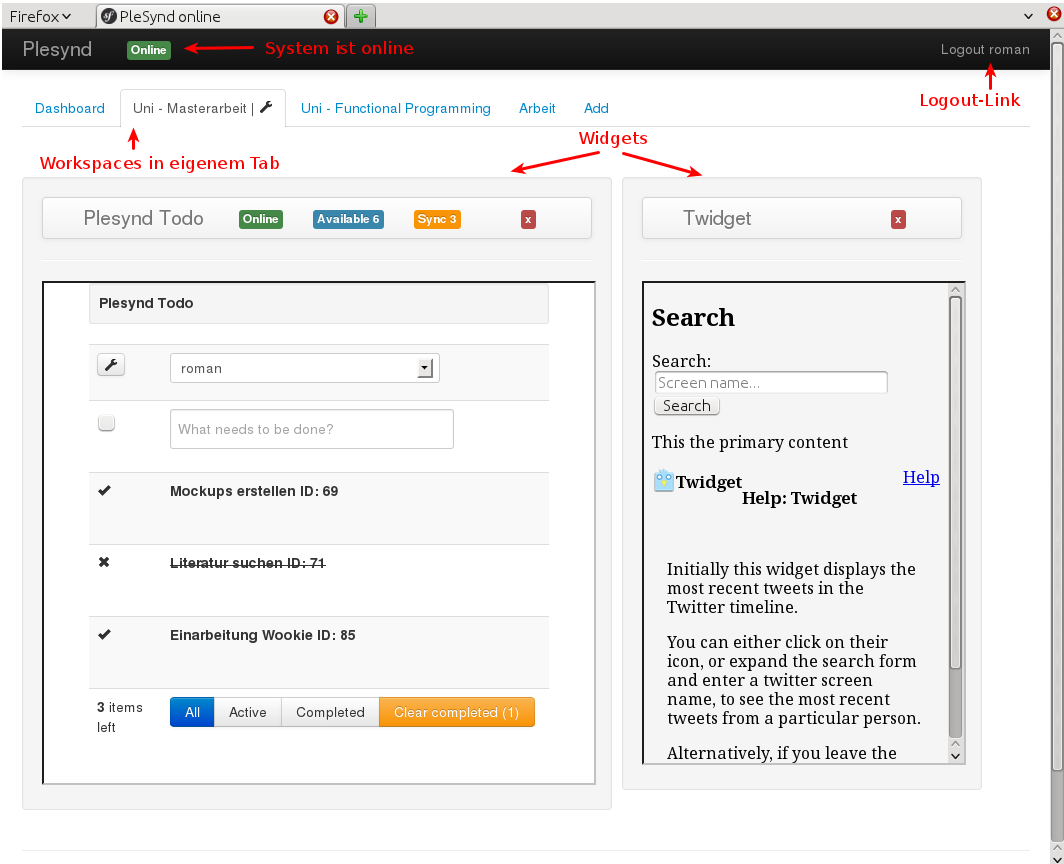
\includegraphics[]{./Figures/plesynd_workspace_online.png}
    \rule{35em}{0.5pt}
  \caption[Plesynd User"=Interface: Workspace Online]{Ein Workspace mit unterschiedlichen Widgets}
  \label{fig:plesynd_workspace_online}
\end{figure}

\begin{figure}
  \centering
  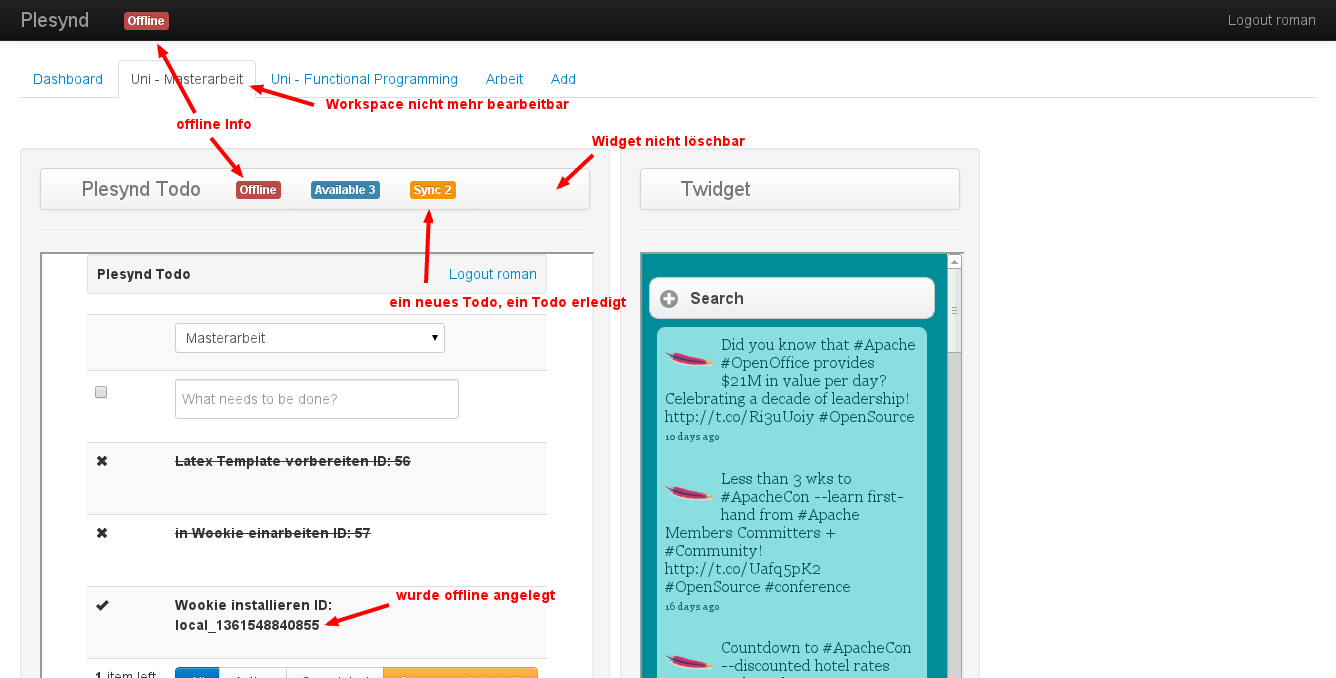
\includegraphics[]{./Figures/plesynd_workspace_offline.png}
    \rule{35em}{0.5pt}
  \caption[Plesynd User"=Interface: Workspace Offline]{Die wichtigsten Unterschiede im Offline"=Modus}
  \label{fig:plesynd_workspace_offline}
\end{figure}

\begin{figure}
  \centering
  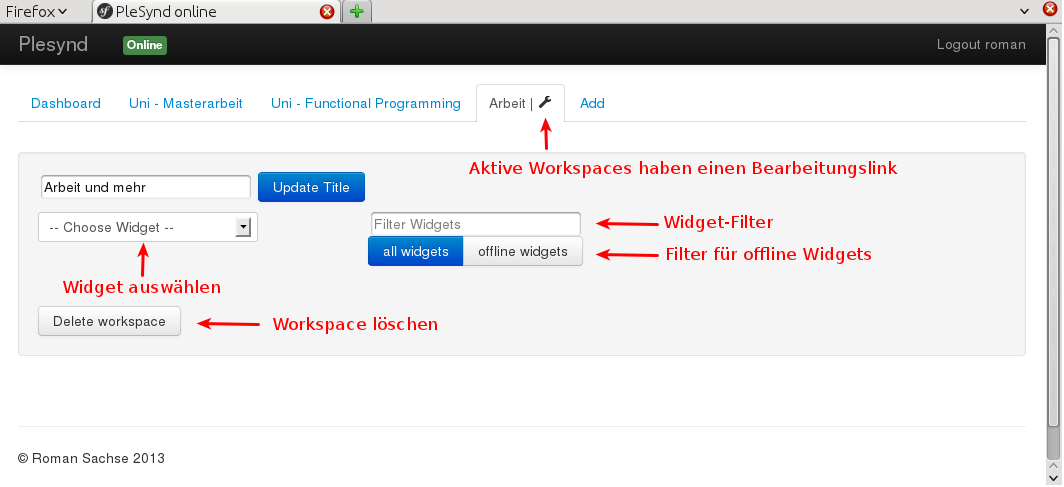
\includegraphics[]{./Figures/plesynd_workspace_edit.png}
    \rule{35em}{0.5pt}
  \caption[Plesynd User"=Interface: Bearbeiten von Workspaces]{Workspaces können direkt bearbeitet werden.}
  \label{fig:plesynd_workspace_edit}
\end{figure}

Zusammenfassend wurde für diese Arbeit mit Plesynd sowohl das Frontend als auch das Backend einer neuen Personal Learning Environment von Grund auf entworfen und auf Basis aktueller Webtechnologien implementiert.
